\section {IMU Cluster}
В настоящее время широкое распространение получили блоки инерциальных чувствительных элементов (БЧЭ) на базе MEMS-технологии.
Их основными преимуществами являются: низкая стоимость, малые массогабаритные характеристики и низкое энергопотребление.
Однако подобные приборы обладают низкой точностью: нестабильность нуля у гироскопов единицы-десятки градусов в час, а у акселерометров сотые-десятые доли милли-g.

Одним из путей повышения точности микромеханических БЧЭ является объединение их в массив (кластер). [ссылки на работы по кластеру].
Кластерные бчэ позволяют уменьшить шум в информационном сигнале в $\sqrt{N}$ раз, где $N$ - количество отдельных используемых бчэ. [ссылка]

\newpage

\begin{figure}[h!]
	\centering
	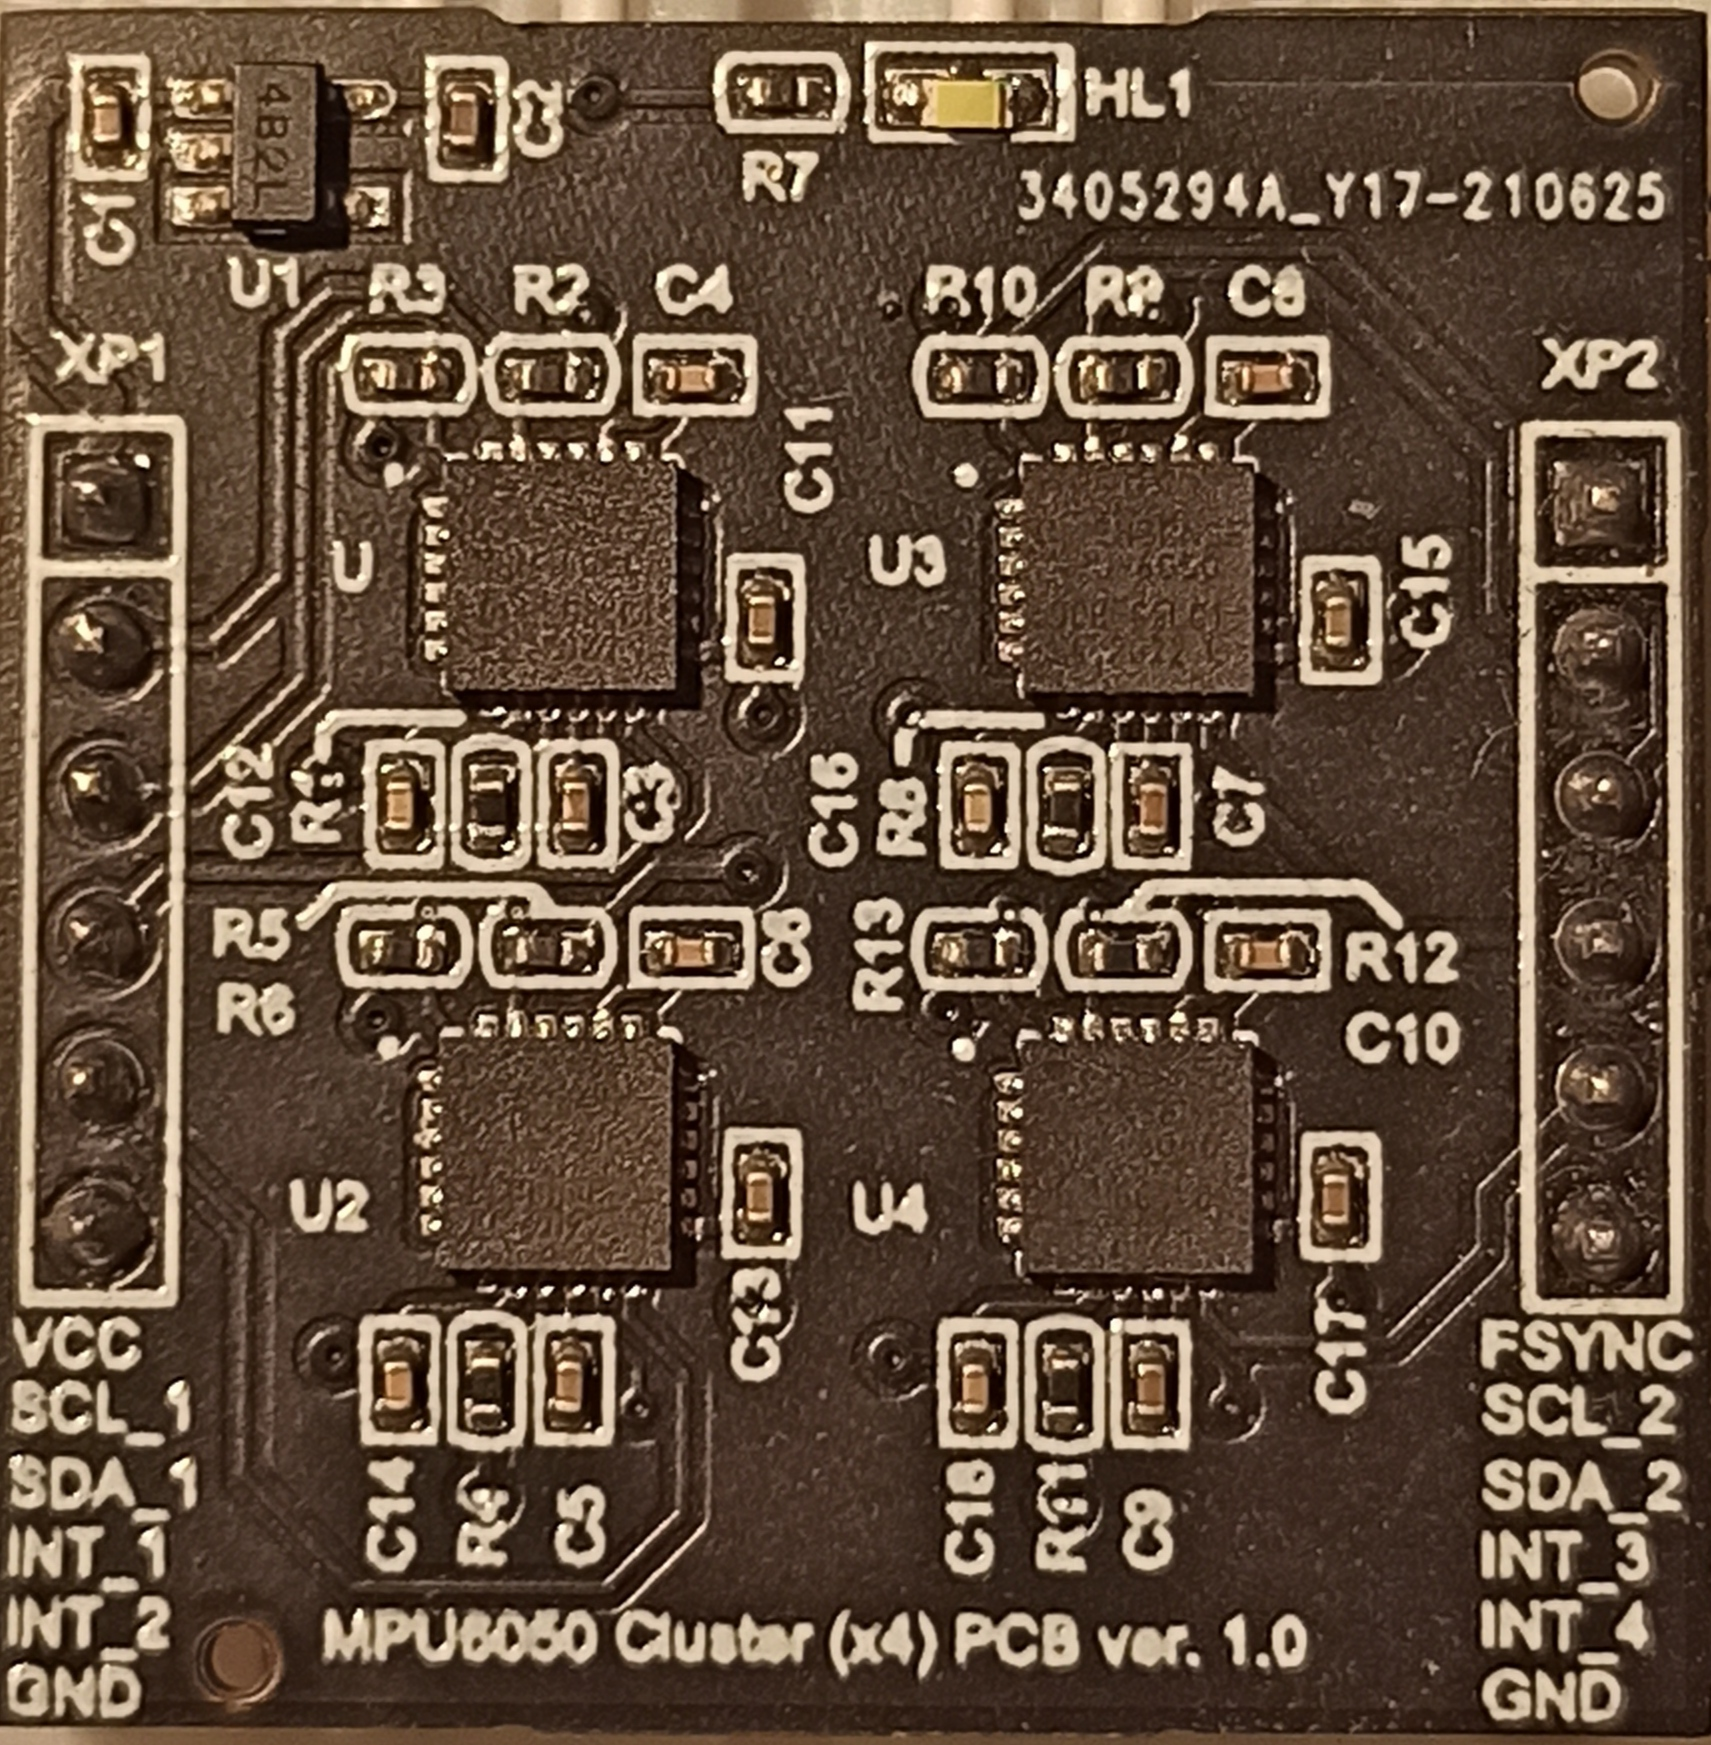
\includegraphics[width=0.3\linewidth]{cluster_pcb.jpg}
	\caption{Печатная плата с кластерным БЧЭ}
	\label{fig:cluster_pcb}
\end{figure}

Для проверки и исследования погрешностей кластерного БЧЭ разработана печатная плата (Рис. \ref{fig:cluster_pcb}).

В состав разработанного кластерного БЧЭ входят шестиосные датчики фирмы Invensense MPU6050 (трехосный акселерометр и трехосный датчик угловых скоростей).
Данные БЧЭ были выбраны вследствие их наибольшей распространнености и доступности.
Каждый из MPU6050 располагается на печатной плате в вершинах квадрата со стороной 10 мм.
Кроме того, они установлены так, чтобы соответствующие оси чувстительности каждого датчика были параллельны между собой.

Для записи данных с чувствительных элементов в составе MPU6050 были использованы следующие характеристики: диапазон измеряемых угловых скоростей $\pm$500 \SI[per-mode=symbol]{}{\degree\per\second};
диапазон измеряемых линейных ускорений $\pm$4g. Съем информации с датчиков производился на частоте 100 Гц.
Данные параметры были выбраны в предположении установки разрабатываемого устройства на маломаневренных, наземных объектах.

%Оценка смещения нуля у используемых датчиков и их дрейфа от запуска к запуску
Для калибровки и оценки смещения нуля и его дрейфа от запуска к запуску были проведены записи данных в шести положениях (Pos. 1 - Z$\uparrow$, Pos.2 - Z$\downarrow$,
Pos. 3 - X$\uparrow$, Pos.4 - X$\downarrow$, Pos. 5 - Y$\uparrow$, Pos.6 - Y$\downarrow$). Для каждого из положений производилось по три запуска, по итогам которых рассчитывались
оцениваемые параметры. Результаты измерений для акселерометров по соответствующим осям одного из БЧЭ сведены в таблицу (\ref{table:acc_rtr}) (для остальных БЧЭ полученные величины отличались незначительно).

\begin{table}[h!]
	\centering
	\caption{Смещение нуля и дрейф от запуска к запуску акселерометров MPU6050}
	\begin{tabular}{|c|c|c|c|}
	\hline
	Position & Axis & Mean, g & RTR, mg \\ \hline
	\multirow{3}{*}{Pos.1}	& X & 0.0686 & 0.068 \\											 
							\cline{2-4}
							& Y & -0.0250 & 0.06 \\												 
							\cline{2-4}
							& Z & 1.0199 & 0.2413 \\												 
	\hline
	\multirow{3}{*}{Pos.2}	& X & 0.0541 & 0.0943 \\												 
							\cline{2-4}
							& Y & -0.0086 & 0.0501 \\												 
							\cline{2-4}
							& Z & -1.0121 & 0.2652 \\												 
	\hline	
	\multirow{3}{*}{Pos.3}	& X & 1.0567 & 0.1836 \\												 
							\cline{2-4}
							& Y & -0.0246 & 0.0878 \\												 
							\cline{2-4}
							& Z & 0.0028 & 0.1113 \\												 
	\hline
	\multirow{3}{*}{Pos.4}	& X & -0.9377 & 0.1664 \\												 
							\cline{2-4}
							& Y & -0.0045 & 0.0966 \\												 
							\cline{2-4}
							& Z & -0.00004 & 0.2716 \\												 
	\hline
	\multirow{3}{*}{Pos.5}	& X & 0.0486 & 0.0729 \\												 
							\cline{2-4}
							& Y & -1.0271 & 0.0152 \\												 
							\cline{2-4}
							& Z & -0.0071 & 0.2099 \\												 
	\hline
	\multirow{3}{*}{Pos.6}	& X & 0.0731 & 0.2276 \\												 
							\cline{2-4}
							& Y & 0.9929 & 0.1313 \\												 
							\cline{2-4}
							& Z & 0.0171 & 0.2973 \\												 
	\hline
	\end{tabular}
	\label{table:acc_rtr}
\end{table}

Аналогичные результаты измерений представлены для гироскопов MPU6050 по соответствующим осям (Таблица (\ref{table:gyr_rtr})).

\begin{table}[h!]
	\centering
	\caption{Смещение нуля и дрейф от запуска к запуску гироскопов MPU6050}
	\begin{tabular}{|c|c|c|c|}
	\hline
	Position & Axis & Mean, \SI[per-mode=symbol]{}{\degree\per\second} & RTR, \SI[per-mode=symbol]{}{\degree\per\hour} \\ \hline
	\multirow{3}{*}{Pos.1}	& X & -1.0739 & 44.8406 \\												 
							\cline{2-4}
							& Y & -1.0022 & 17.3611 \\												 
							\cline{2-4}
							& Z & 1.2711 & 22.4487 \\												 
	\hline
	\multirow{3}{*}{Pos.2}	& X & -1.0246 & 59.2236 \\												 
							\cline{2-4}
							& Y & -0.9897 & 15.8603 \\												 
							\cline{2-4}
							& Z & 1.2628 & 27.1911 \\												 
	\hline	
	\multirow{3}{*}{Pos.3}	& X & -1.0122 & 66.8934 \\												 
							\cline{2-4}
							& Y & -0.9913 & 16.7310 \\												 
							\cline{2-4}
							& Z & 1.2515 & 34.0154 \\												 
	\hline
	\multirow{3}{*}{Pos.4}	& X & -1.0254 & 17.4720 \\												 
							\cline{2-4}
							& Y & -0.9991 & 7.7416 \\												 
							\cline{2-4}
							& Z & 1.2946 & 12.8763 \\												 
	\hline
	\multirow{3}{*}{Pos.5}	& X & -1.0106 & 13.5531 \\												 
							\cline{2-4}
							& Y & -0.9849 & 3.7527 \\												 
							\cline{2-4}
							& Z & 1.2519 & 7.4237 \\												 
	\hline
	\multirow{3}{*}{Pos.6}	& X & -1.0095 & 1.7701 \\												 
							\cline{2-4}
							& Y & -0.9878 & 12.9651 \\												 
							\cline{2-4}
							& Z & 1.2655 & 19.6326 \\												 
	\hline
	\end{tabular}
	\label{table:gyr_rtr}
\end{table}

Исходя из полученных значений, можно сделать вывод, что дрейф от запуска к запуску для акселерометров (max $\approx$0.3 mg) и гироскопов (max $\approx$70 \SI[per-mode=symbol]{}{\degree\per\hour}) невелик.
Это значит, что полученные оценки смещений нуля можно использовать для калибровки БЧЭ при дальнейшей работе.

%Оценка шумовых характеристик используемых датчиков по методу вариации Аллана
Также была проведена оценка шумовых характеристик микромеханических чувствительных элементов в составе MPU6050 по методу вариации Аллана. [IEEE 1431-2004, IEEE 1293-2018]
Для этого данные были записаны в течение одного часа в Pos. 1. На рисунке \ref{fig:acc_y_allan} продемонстрированы результаты расчета девиации Аллана акселерометров по оси чувствительности Y.
График с точками в виде ромбов отражает расчет девиации Аллана для кластерного БЧЭ. Расположение данного графика ниже остальных подтверждает уменьшение шума в сигнале кластерного БЧЭ 
по сравнению с сигналом единичного БЧЭ.

%Графики девиации Аллана для акселерометров по каналу Y. Сводная таблица погрешностей акселерометров.
\begin{figure}[h!]
	\centering
	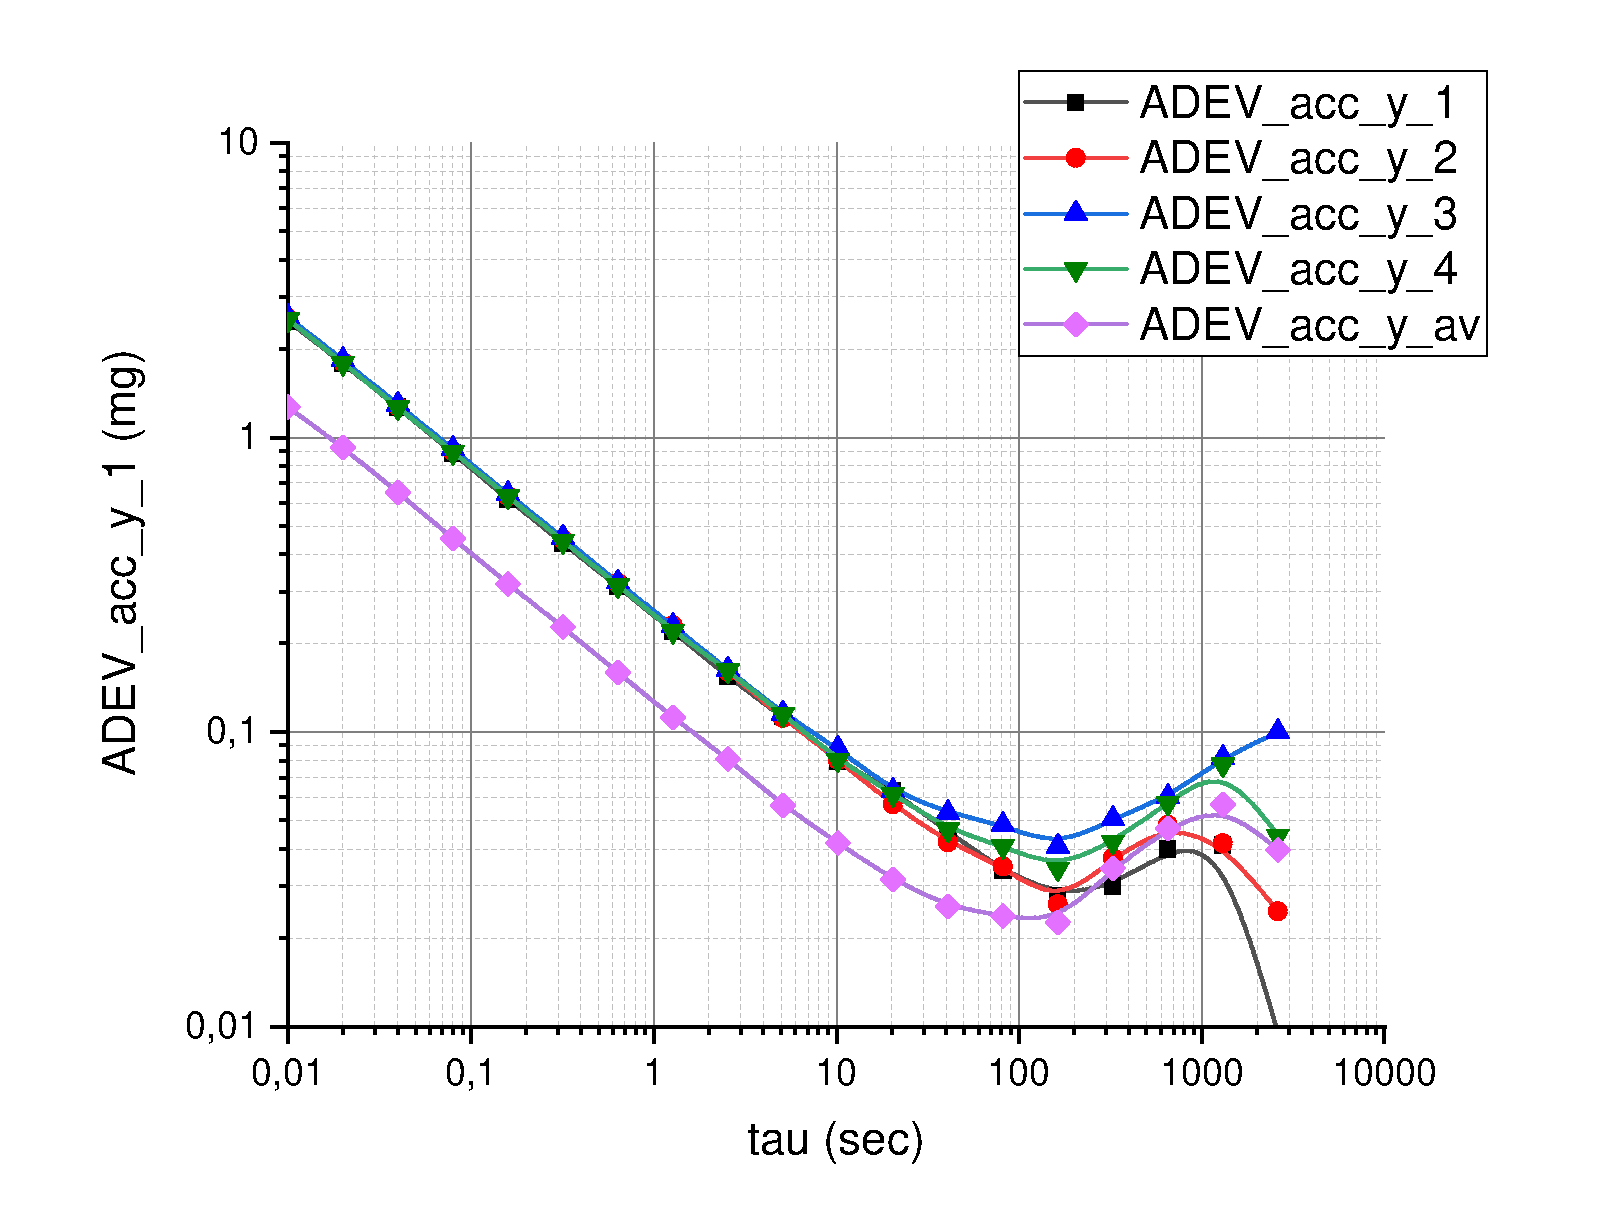
\includegraphics[width=0.7\linewidth]{acc_y_adev.pdf}
	\caption{Девиация Аллана акселерометров по оси Y}
	\label{fig:acc_y_allan}
\end{figure}

\newpage

В таблицах \ref{table:acc_bias} and \ref{table:acc_vrw} представленны численные значения оценок Bias instability and Velocity Random Walk for accelerometers.

\begin{table}[h!]
	\centering
	\begin{tabular}{| c | c | c | c | c | c |}
	\hline
	Ось & IMU\_1 & IMU\_2 & IMU\_3 & IMU\_4 & Cluster \\ \hline
	X & 0.0467 & 0.0409 & 0.0417 & 0.0417 & 0.0264 \\ \hline
	Y & 0.0278 & 0.0259 & 0.0409 & 0.0344 & 0.0225 \\ \hline
	Z & 0.0764 & 0.0704 & 0.0714 & 0.0692 & 0.0472 \\
	\hline
	\end{tabular}
	\caption{Нестабильность смещения нуля акселерометров MPU6050, mg}
	\label{table:acc_bias}
\end{table}

\begin{table}[h!]
	\centering
	\begin{tabular}{| c | c | c | c | c | c |}
	\hline
	Ось & IMU\_1 & IMU\_2 & IMU\_3 & IMU\_4 & Cluster \\ \hline
	X & 0.24014 & 0.22564 & 0.24332 & 0.24124 & 0.11715 \\ \hline
	Y & 0.22065 & 0.23029 & 0.22929 & 0.22040 & 0.11211 \\ \hline
	Z & 0.35402 & 0.35872 & 0.36701 & 0.37358 & 0.18599 \\
	\hline
	\end{tabular}
	\caption{Velocity random walk (VRW) of accelerometers MPU6050, mg/$\sqrt{Hz}$}
	\label{table:acc_vrw}
\end{table}

%Выводы по данным из таблицы
Полученные результаты подтверждают гипотезу, что шумовые характеристики сигнала для акселерометров кластерного БЧЭ в $\approx\sqrt{4} = 2$ раза меньше по сравнению с характеристиками каждого
из акселерометров по отдельности.

Аналогичные оценки шума были проведены и для гироскопов в составе кластерного БЧЭ. На рисунке \ref{fig:gyr_y_allan} представлены девиации Аллана гироскопов по оси чувствительности Y.
График девиации Аллана для сигнала, полученного путем усреднения данных по четырем сигналам гироскопов (diamond) также располагается ниже графиков для каждого из гироскопов по отдельности.

%Графики девиации Аллана для гироскопов по каналу Y. Сводная таблица погрешностей гироскопов.
\begin{figure}[h!]
	\centering
	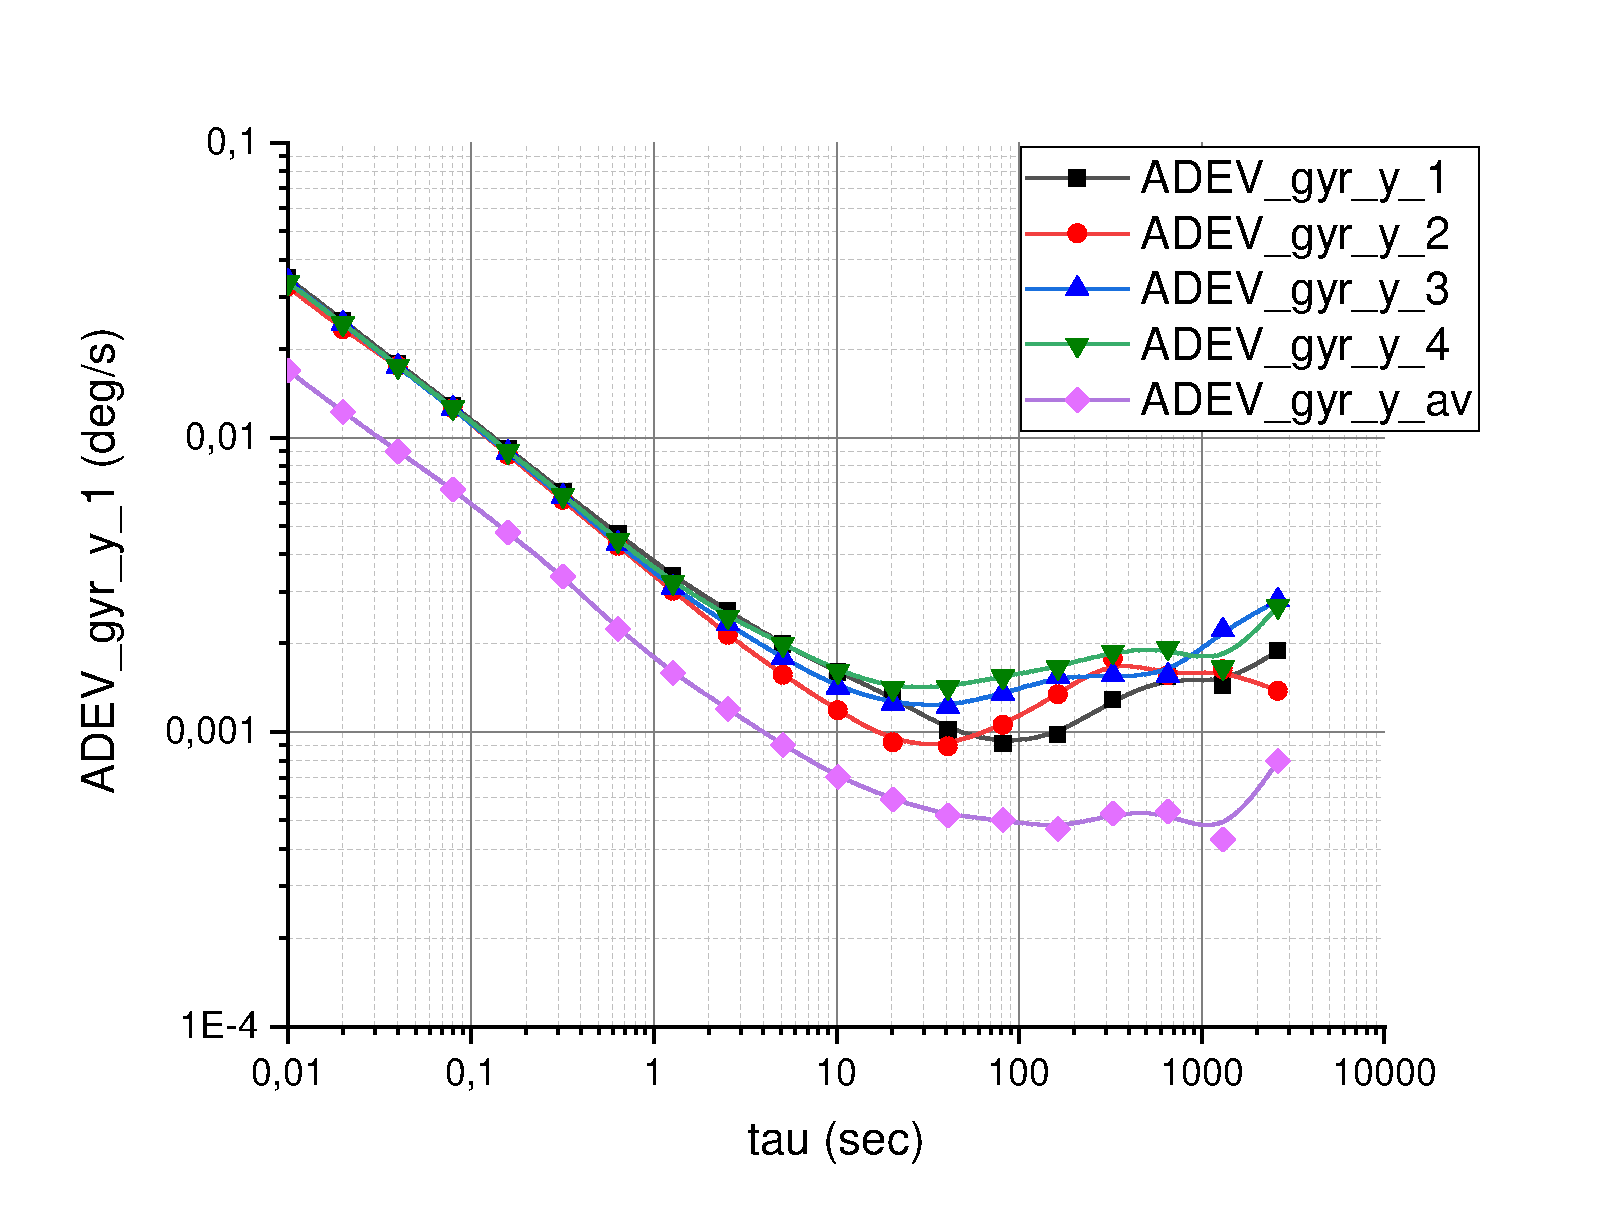
\includegraphics[width=0.7\linewidth]{gyr_y_adev.pdf}
	\caption{Девиация Аллана гироскопов по оси Y}
	\label{fig:gyr_y_allan}
\end{figure}

В таблицах \ref{table:gyro_bias} and \ref{table:gyro_arw} собраны численные значения оценок Bias instability and Angular Random Walk for gyroscopes.

\begin{table}[h!]
	\centering
	\caption{Нестабильность смещения нуля гироскопов MPU6050, \SI[per-mode=symbol]{}{\degree\per\hour}}
	\begin{tabular}{| c | c | c | c | c | c |}
	\hline
	Ось & IMU\_1 & IMU\_2 & IMU\_3 & IMU\_4 & Cluster \\ \hline
	X & 4.644 & 3.553 & 3.780 & 4.327 & 2.416 \\ \hline
	Y & 3.272 & 3.215 & 4.370 & 5.087 & 1.685 \\ \hline
	Z & 3.740 & 2.696 & 3.503 & 2.693 & 1.580 \\
	\hline
	\end{tabular}
	\label{table:gyro_bias}
\end{table}

\begin{table}[h!]
	\centering
	\caption{Angular random walk (ARW) of gyroscopes MPU6050, \SI[per-mode=symbol]{}{\degree}/$\sqrt{hr}$}
	\begin{tabular}{| c | c | c | c | c | c |}
	\hline
	Ось & IMU\_1 & IMU\_2 & IMU\_3 & IMU\_4 & Cluster \\ \hline
	X & 0.2022 & 0.1872 & 0.2382 & 0.2010 & 0.1044 \\ \hline
	Y & 0.2028 & 0.1812 & 0.1854 & 0.1938 & 0.0954 \\ \hline
	Z & 0.1638 & 0.2106 & 0.1884 & 0.1944 & 0.0972 \\
	\hline
	\end{tabular}
	\label{table:gyro_arw}
\end{table}

%Выводы по данным таблицы
Полученные характеристики для кластерного сигнала гироскопов также в $\approx2$ раза меньше величин для каждого из гироскопов по отдельности.

Таким образом, изготовленный макет подтвердил свойства кластерных БЧЭ, позволяя улучшить параметры, используемых MPU6050 в $\approx2$ раза.

\newpage